\chapter*{Preface}


%citazione introduttiva
\epigraph{\textit{How do we know what we know?}}{}

Thousands of years ago, the Greek philosopher Plato introduced the “theory of \textit{Forms}”, i.e. a philosophical viewpoint where an ideal world called \textit{Hyperuranion} contains the purest and most accurate realisation of the knowledge. This unreachable knowledge is called the \textit{Form}. The reality surrounding us in the real world is an imitation of the \textit{Form}, and it is called the \textit{Substance}. Then, according to Plato, knowledge is a deductive process, from the steady and perfect Form to its “dirty” realisation in the \textit{Substance}.\par

Differently, the Greek Philosopher Aristotle considers the real world as the only source of knowledge. In his viewpoint, the empirical process of observing the world is the path to get knowledge. This process is, then, inductive and implies that anything can only exist if a living being can observe it.\par

Aristotle’s philosophy is the background of this work that will approach the logistics and operations phenomena with an inductive approach. The data-driven methodology creating knowledge by observing and classifying data is an implementation on lifeless machines of one of the most beautiful philosophical intuition in the story of our world.\par

% INSERT fig_actors

\begin{figure}[hbt!]
\centering
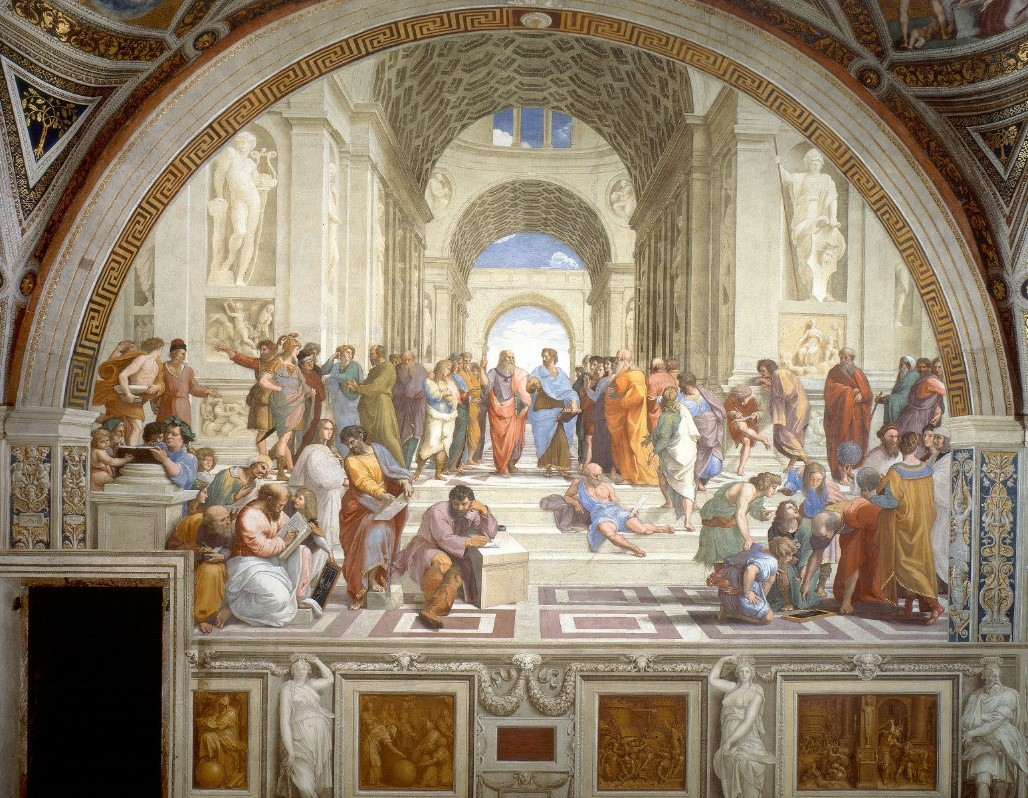
\includegraphics[width=0.9\textwidth]{other/preface_figures/laScuolaDiAtene.jpg}
\captionsetup{type=figure}
\caption{“The school of Athens”, Apostolic Palace, Vatican City. In the centre of the fresco, Plato and Aristotle.}
\end{figure}
